Il Dataset utilizzato allo scopo è stato preso dalla piattaforma Kaggle\footnote{\href{https://www.kaggle.com/datasets/ankurzing/sentiment-analysis-for-financial-news}{Kaggle dataset: sentiment-analysis-for-financial-news}} e consiste in 4846 news headlines annotate con tre classi (sentiment), che indica quanto il titolo finanziario in questione è appetibile da parte di un possibile investitore. Le tre classi sono rispettivamente positivo (28.1\% sul totale del dataset), negativo (12.5\%) e neutrale (59.4\%).

\begin{figure}[!ht]
    \centering
    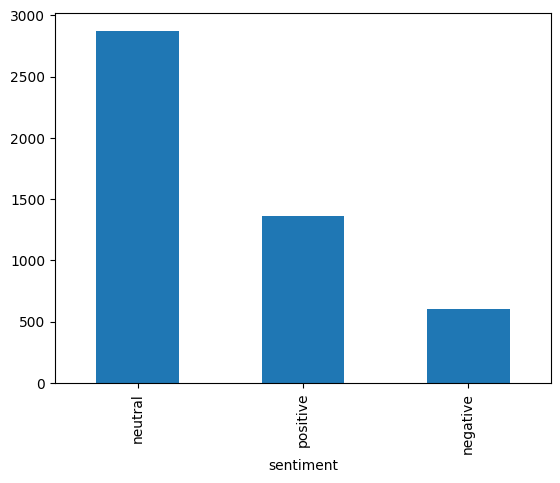
\includegraphics[width=10cm]{./images/dataset_percentage_bar_plot.png}
    \caption{Sample occurencies bar plot per class }
\end{figure}

\newpage



